\chapter{Planificación, metodología y presupuesto del proyecto}\label{cap:planificacion}

En este apartado se presenta la planificación del proyecto, incluyendo el cronograma de trabajo, la metodología de desarrollo utilizada y la gestión de riesgos.

\section{Cronograma del proyecto}

Antes del comienzo del desarrollo del proyecto, se realizó una planificación inicial que incluía la definición de los sprints y las tareas a realizar en cada uno de ellos de manera general, definiendo hitos, no tareas específicas. Esta planificación se ha seguido a lo largo del desarrollo, aunque ha habido ajustes en función de los avances y los resultados obtenidos.

La realización del cronograma se ha llevado a cabo haciendo uso de la herramienta \textbf{GantPRO}\cite{webGanttPro}, que permite la creación de diagramas de Gantt de manera sencilla y efectiva. A continuación, se presenta el diagrama de Gantt del proyecto, que muestra las diferentes fases y tareas a realizar en cada sprint.

\begin{figure}[ht!] 
    \centering 
    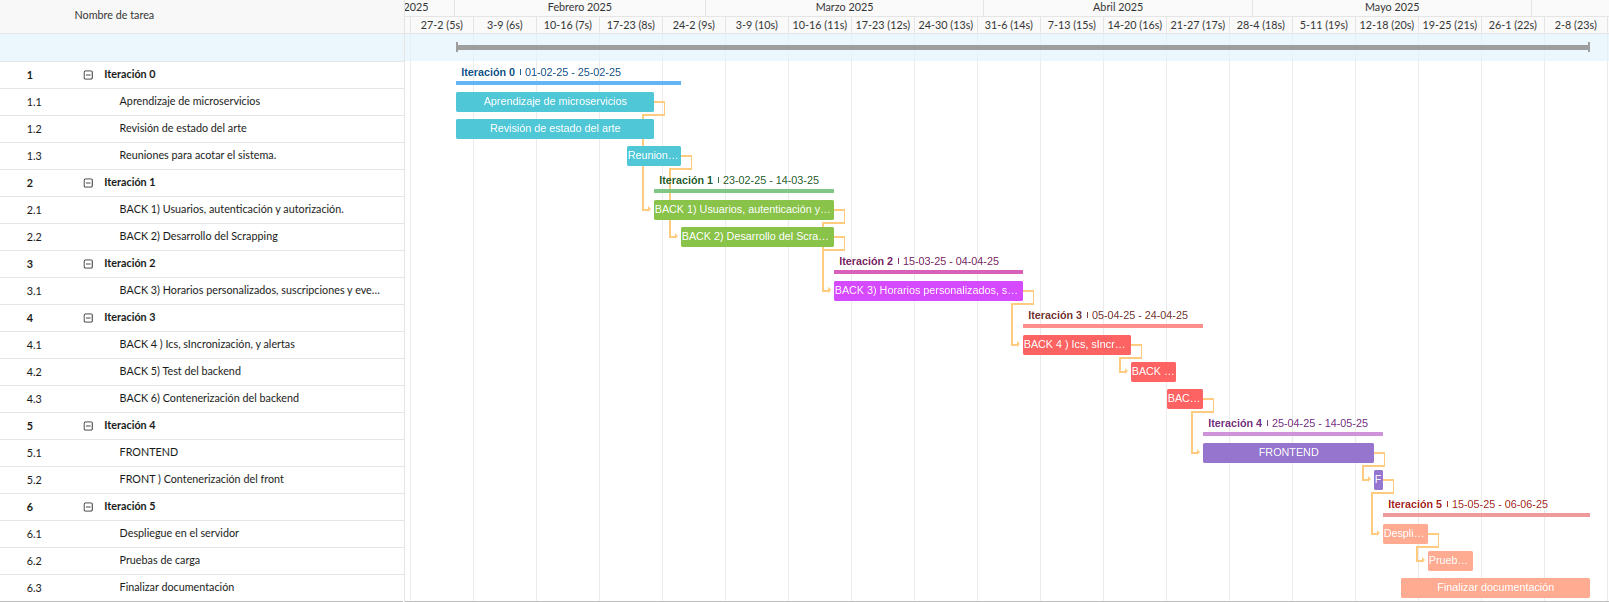
\includegraphics[width=1\textwidth]{figures/04_gantt.png}
    \caption{Gantt del proyecto.} 
    \label{gantt}
\end{figure}

El cronograma del proyecto se ha dividido en 5 sprints, cada uno con una duración de 3 semanas. Como se muestra en la figura \ref{gantt}, cada sprint ha tenido un conjunto de tareas generales a realizar, que se han ido completando a lo largo del desarrollo.

\begin{enumerate}
    \item \textbf{Sprint 0:} En este sprint se paraleliza por un lado el aprendizaje técnico acerca de microservicios, docker y el framework de desarrollo backend Spring Boot, a la vez que se acota el sistema y se recaban los requisitos iniciales del sistema.
    \item \textbf{Sprint 1:} En este sprint se comienza el desarrollo del backend implementando los servicios relativos a los usuarios, y la autenticación y autorización basadas en las credenciales de la UGR junto al servicio de mensajería (notificaciones). Además se implementa el scrapping de la we de ``Grados UGR'' para obtener los horarios de los grados.
    \item \textbf{Sprint 2:} En este sprint se continúa el backend implementando las funcionalidades relativas a suscripciones, horarios personalizados y creación de eventos.
    \item \textbf{Sprint 3:} En este sprint se desarrolla la parte del backend relacionada con generación de archivos ics, sincronización con sistemas de calendarios externos y alertas. Además se realizan tests y la contenerización del sistema.
    \item \textbf{Sprint 4:} En este sprint se desarrolla el frontend del sistema, implementando la interfaz de usuario y la comunicación con el backend.
    \item \textbf{Sprint 5:} En este último sprint se realiza el despliegue en el servidor de la UGR, se realizan pruebas de carga y se finaliza el proyecto para su entrega. Además se añade la funcionalidad extra de búsqueda de suscripciones por nombre de profesor, de modo que podemos suscribirnos directamente a los grupos de aasignaturas que imparte este.
\end{enumerate}

En todos los sprints se realizarán además tareas de documentación y pruebas, además del seguimiento y registro de horas dedicadas a cada tarea.

\section{Metodología de desarrollo}
Para la gestión y desarrollo del proyecto, se ha optado por la metodología ágil \hyperlink{scrum}{Scrum}. Esta metodología se caracteriza por su enfoque iterativo e incremental, permitiendo una adaptación flexible a los cambios y una entrega temprana de valor.

\subsection{Roles y Responsabilidades en este Proyecto}

Dada la naturaleza individual de este proyecto, los roles tradicionales de Scrum se han adaptado de la siguiente manera:

\begin{itemize}
    \item \textbf{Equipo de Desarrollo y Scrum Master:} El autor de este TFG ha asumido ambos roles. Esto implica la responsabilidad de llevar a cabo el desarrollo del software, así como de facilitar el proceso Scrum, asegurando que se sigan las prácticas y principios de la metodología. Se ha encargado de la planificación, ejecución y revisión de cada sprint, así como de la identificación y resolución de impedimentos.
    \item \textbf{Product Owner:} El rol de Product Owner ha sido desempeñado tanto por el director del TFG, D. Juan Luis Jiménez Laredo, como por el autor del sistema. En esta función, ambos han sido los responsables de definir la visión del producto, priorizar el Backlog del Producto y asegurar que el desarrollo se alinee con las necesidades y expectativas del proyecto. Los dos participaron activamente en la definición de los requisitos y en la validación de los incrementos de software.
\end{itemize}

\subsection{Proceso Scrum Implementado}

El proceso Scrum se ha implementado siguiendo los siguientes pasos clave:

\begin{itemize}
    \item \textbf{\hyperlink{backlog}{Backlog} del Producto:} Se ha definido un Backlog del Producto inicial, compuesto por las funcionalidades y tareas necesarias para completar el TFG.
    \item \textbf{Sprints:} El desarrollo se ha dividido en 5 sprints de duración 3 semanas cada uno. Cada sprint ha tenido como objetivo la entrega de un incremento de software funcional y potencialmente entregable.
    \item \textbf{Planificación del Sprint:} Al inicio de cada sprint, se ha llevado a cabo una reunión de planificación en la que, junto con el Product Owner, se han seleccionado los elementos del Backlog del Producto que se abordarían durante el sprint. Se han estimado las tareas y se ha definido el Sprint Backlog.
    \item \textbf{Desarrollo del Sprint:} Durante el sprint, el autor ha trabajado en el desarrollo de las tareas asignadas, siguiendo las prácticas de desarrollo y asegurando la calidad del código.
    \item \textbf{Reunión Diaria (Daily Scrum):} Aunque adaptada a la naturaleza individual del proyecto, se ha realizado una reflexión diaria sobre el progreso, los impedimentos y las tareas a realizar. Esto ha permitido mantener un seguimiento constante del avance.
    \item \textbf{Revisión del Sprint (Sprint Review):} Al finalizar cada sprint, se ha llevado a cabo una revisión del sprint. Dado que el autor es también el equipo de desarrollo, esta revisión ha consistido en una \textbf{introspección personal y un análisis de los resultados del sprint}, evaluando las metas alcanzadas y el incremento de software desarrollado. Se ha realizado una autoevaluación del progreso y la calidad del trabajo.
    \item \textbf{Retrospectiva del Sprint (Sprint Retrospective):} La retrospectiva del sprint se ha realizado en colaboración con el Product Owner (D. Juan Luis Jiménez Laredo). En esta reunión, se ha analizado el sprint finalizado, identificando qué se ha hecho bien, qué se podría mejorar y qué acciones concretas se podrían implementar para el siguiente sprint. Esta colaboración ha permitido obtener una perspectiva externa y valiosa para la mejora continua del proceso.
\end{itemize}

\subsection{Justificación de la Metodología}

La elección de la metodología Scrum se justifica por las siguientes razones:

\begin{itemize}
    \item \textbf{Flexibilidad:} Permite adaptarse a los cambios en los requisitos y a los aprendizajes obtenidos durante el desarrollo. En concreto este sistema dependía en etapas tempranas de desarrollo del posible acceso a datos oficiale de la UGR, sistemas de autenticación internos, datos de matriculaciones, etc. Es por ello que la flexibilidad de Scrum ha sido clave para ajustar el plan a medida que se han ido conociendo más detalles.
    \item \textbf{Entrega Temprana de Valor:} Facilita la entrega de incrementos funcionales de software de forma regular, lo que permite obtener retroalimentación temprana y ajustar el rumbo del proyecto si es necesario.
    \item \textbf{Transparencia:} El uso de herramientas como GitHub Projects y la realización de las reuniones Scrum promueven la transparencia en el progreso del proyecto.
    \item \textbf{Adaptabilidad a un Proyecto Individual:} Aunque tradicionalmente Scrum se aplica a equipos, su estructura iterativa y adaptable se ajusta bien a un proyecto individual como un TFG, permitiendo una organización eficiente del trabajo y una gestión del tiempo efectiva.
\end{itemize}

Es importante destacar que, dada la naturaleza individual del proyecto, se ha realizado una adaptación de los roles y las ceremonias de Scrum para ajustarse a las necesidades y recursos disponibles. 
Sin embargo, se han mantenido los principios fundamentales de la metodología para asegurar una gestión eficaz del desarrollo.

\subsection{Gestión de Tareas y Seguimiento del Progreso}

Para la gestión de las tareas y el seguimiento del progreso del proyecto, se ha utilizado \textbf{GitHub Projects}\cite{calendarugr_github}. Esta herramienta ha permitido:

\begin{itemize}
    \item \textbf{Creación de un Backlog del Producto:} Se ha creado un backlog del producto en GitHub Projects, donde se han definido las historias de usuario y las tareas necesarias para el desarrollo del sistema. Este backlog ha sido la base para la planificación de los sprints y la gestión de las tareas.
    \newline\newline
    Cada tarea creada en este ha representado una historia de usuario o una tarea aparte a realizar ( reuniones, investigación, etc.). Cada tarea ha sido asignada a un sprint y se ha estimado el tiempo necesario para su realización usando la técnica de \textbf{``Planning Poker''}. Esta técnica ha permitido una estimación más precisa y consensuada entre el Product Owner y el equipo de desarrollo.
    Además cada historia de usuario conllevaba una seriie de criterios de aceptación que se han ido marcando a medida que se iban cumpliendo. 
    
    \begin{figure}[H] 
        \centering 
        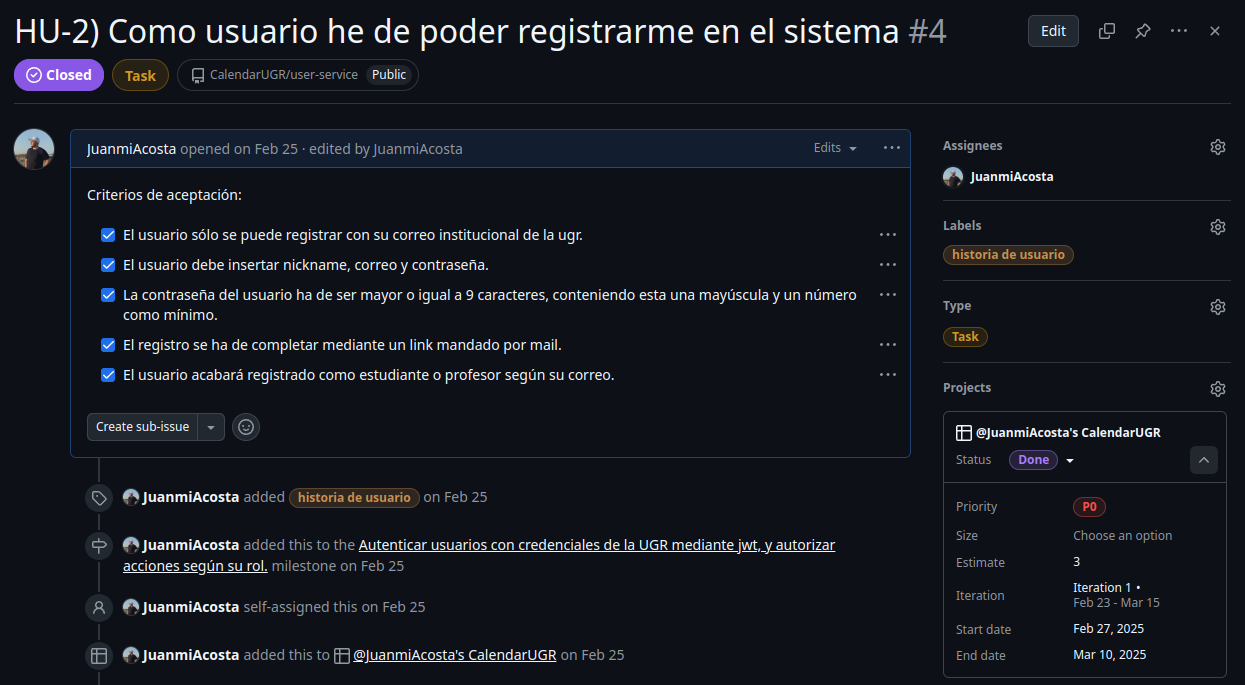
\includegraphics[width=0.9\textwidth]{figures/05_hu.png}
        \caption{Ejemplo de historia de usuario en Github Projects.} % Leyenda de la imagen
        \label{historia de usuario} % Etiqueta para referenciar la imagen
    \end{figure}

    \item \textbf{Creación de Tableros por Sprint:} Se han configurado tableros de proyecto en GitHub Projects, utilizando las funcionalidades de \textbf{``Iteraciones''} para representar cada sprint. Esto ha facilitado la visualización del trabajo en curso para cada iteración.
    \newline
    Antes del comienzo de cada sprint se revisa el product backlog, se seleccionan las tareas a realizar y se crea el tablero correspondiente poniendo todas las tareas en estado ``To do''. Además también se revisan las prioridades de estas y se cambian si el proyecto lo requiere.
    Durante el desarrollo del sprint, las tareas se van moviendo a los diferentes estados según su avance ( ``Backlog'', ``Todo'', ``In progress'', ``Testing'', ``Done'').
    
    \begin{figure}[H] 
        \centering 
        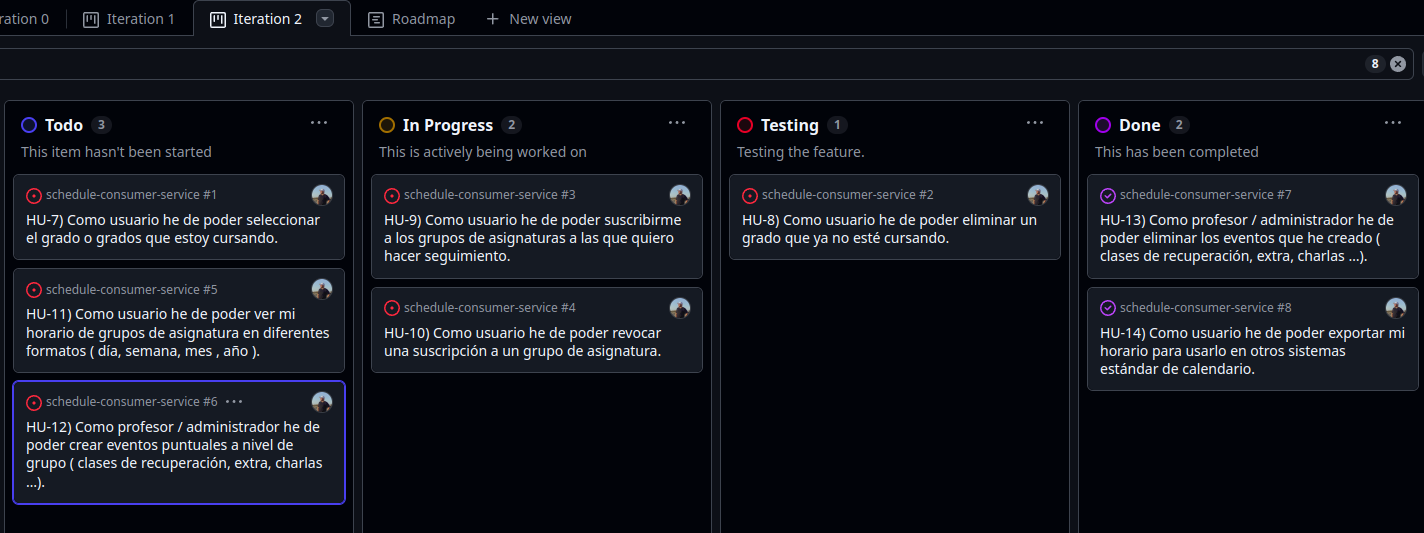
\includegraphics[width=1\textwidth]{figures/04_github_tablero.png}
        \caption{Tablero del 2º Sprint durante su desarrollo.} % Leyenda de la imagen
        \label{tablero_github} % Etiqueta para referenciar la imagen
    \end{figure}
    
    \item \textbf{Visualización de las tareas en el tiempo:} La herramienta ha permitido visualizar el progreso de las tareas en el tiempo a través de un roadmap, lo que ha facilitado la identificación de posibles retrasos y la toma de decisiones para ajustar el plan si es necesario.
    \newline\newline
    Además este cronograma se ha ido actualizando a medida que se iban completando las tareas, permitiendo una visualización clara del progreso del proyecto, y una escenificación de las tareas realizadas en el tiempo.\newline Enlace al roadmap del proyecto \cite{roadmap}.

    \begin{figure}[H] 
        \centering 
        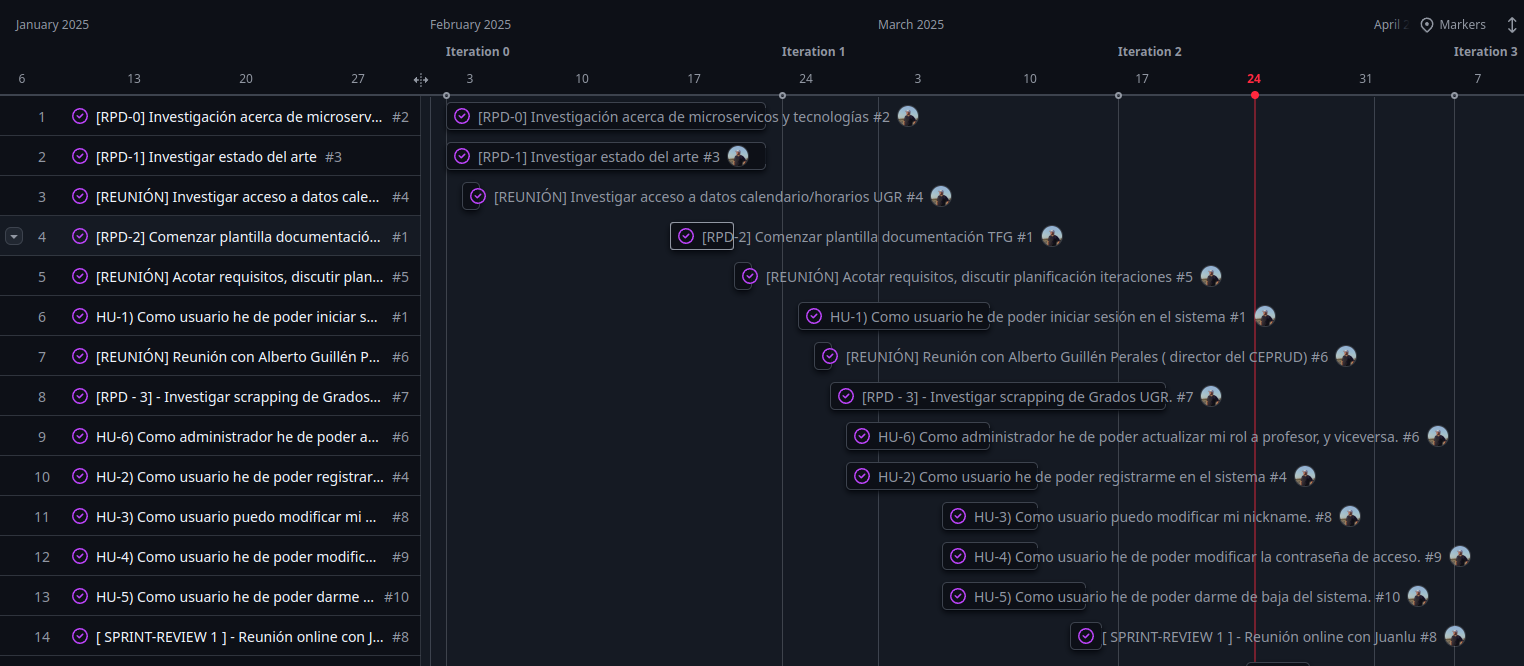
\includegraphics[width=1\textwidth]{figures/04_roadmap.png}
        \caption{Segmento del ''Roadmap'' del proyecto.} % Leyenda de la imagen
        \label{roadmap_github} % Etiqueta para referenciar la imagen
    \end{figure}
\end{itemize}

Para la gestión del tiempo dedicado a cada tarea, se ha utilizado la funcionalidad de \textbf{``Time Tracking''} Clockify. Esta funcionalidad permite registrar el tiempo dedicado a cada tarea y generar informes sobre el progreso del proyecto. Además, se ha utilizado la técnica de \textbf{``Pomodoro''} para gestionar el tiempo de trabajo, lo que ha permitido mantener un enfoque constante y evitar la fatiga.
\newline\newline
\textbf{Clockify}\cite{clockify} es una herramienta de seguimiento del tiempo que permite registrar el tiempo dedicado a cada tarea y generar informes sobre el progreso del proyecto. Esta herramienta ha sido utilizada para llevar un control detallado del tiempo invertido en cada tarea, lo que ha facilitado la gestión del tiempo y la identificación de posibles retrasos.
Además nos facilita un total de horas dedicadas al desarrollo del proyecto, por lo que facilita demostrar el esfuerzo realizado en el mismo.

\begin{figure}[H] 
    \centering 
    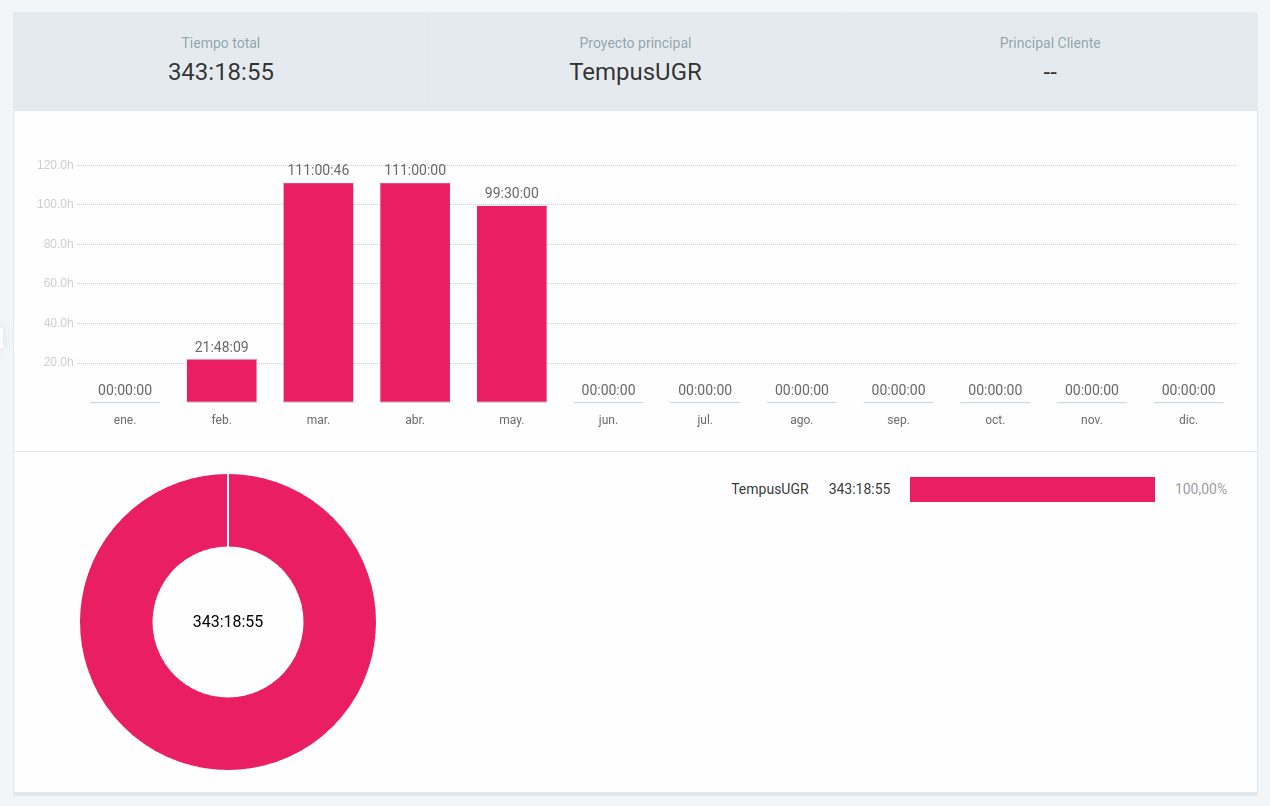
\includegraphics[width=0.8\textwidth]{figures/05_clockify.png}
    \caption{Resumen de horas de desarrollo en Clockify.} % Leyenda de la imagen
    \label{clockify} % Etiqueta para referenciar la imagen
\end{figure}

Este resumen de horas son las correspondientes a los sprints del 1 al 5, e incluye las horas dedicadas a tareas de desarrollo, investigación, reuniones y documentación. En total, y sumando 28.5 horas del curso de microservicos, 5 horas de investigación inicial, y otras 5 horas de reuniones en la iteración 0, se han dedicado un total de 376.5 horas al desarrollo del proyecto.

\section{Desarrollo y control de versiones}

El desarrollo del proyecto se ha realizado utilizando el sistema de control de versiones \textbf{Git} y la plataforma de alojamiento de código \textbf{GitHub}. Esta combinación ha permitido llevar un control detallado de los cambios realizados en el código, facilitar la colaboración y mantener una trazabilidad completa del desarrollo.
\newline\newline
Cada servicio independiente del backend ha supuesto un repositorio independiente, puesto que son programas independientes que se comunican a través de la red. Además se ha creado un repositorio para el frontend y otro para la documentación en latex.
\newline\newline
En este último repositorio se ha hecho uso de \textbf{``Github Actions''} para automatizar el proceso de compilación y despliegue de la documentación, lo que ha permitido mantenerla actualizada de manera continua. Cada vez que se realiza un cambio en la documentación, se ejecuta un flujo de trabajo que compila el código LaTeX y genera el PDF final, asegurando que siempre se disponga de la versión más reciente.
\newline
Además cuando el director de este proyecto ha reflejado aluna corrección mediante comentarios en latex, se ha hecho uso de la funcionalidad de \textbf{``Pull Requests''} de GitHub para revisar y aplicar estos cambios de manera controlada. Esto ha permitido mantener un flujo de trabajo ordenado y garantizar que todas las modificaciones se integren correctamente en la documentación final.

\section{Gestión de riesgos}

En todo proyecto de desarrollo de software, es fundamental identificar y gestionar los riesgos que pueden afectar al éxito del mismo. A continuación se presentan los principales riesgos identificados en este proyecto, junto con las estrategias de mitigación implementadas:

\begin{itemize}
    \item \textbf{Riesgo de cambios en los requisitos:} Dado que desde la el principio del proyecto se trabajó con incertidumbre respecto a la información de la que se podía disponer ( información de los horarios académicos, matriculaciones del alumnado, autenticación institucional ...) y la posibilidad de acceso a estos datos, se ha optado por una metodología ágil (Scrum) que permite adaptarse a los cambios en los requisitos de manera flexible. Además, se ha mantenido una comunicación constante con el Product Owner para ajustar el backlog del producto según sea necesario.
    \newline\newline Además se ha ido ajustando y equilibrando las tareas a realizar entre los sprints, de manera que se realizaban las tareas más prioritarias que eran más difícil que cambiaran con el paso del tiempo, y se dejó para el final ciertas tareas que no estaban tan definidas.

    \item \textbf{Riesgo de problemas técnicos:} Durante el desarrollo del proyecto, se han presentado diversos problemas técnicos relacionados con la implementación de microservicios, la integración de APIs y la contenerización del sistema. Para mitigar este riesgo, se ha realizado una investigación exhaustiva sobre las tecnologías utilizadas y se han seguido buenas prácticas de desarrollo. Además, se ha mantenido una documentación detallada del proceso de desarrollo para facilitar la resolución de problemas.
    \newline\newline En caso de que se presentaran problemas técnicos que no pudieran resolverse, se ha mantenido una comunicación constante con el director del TFG para buscar soluciones y alternativas.

    \item \textbf{Imposibilidad de cumplir con los plazos establecidos:} Dada la naturaleza individual del proyecto, existe el riesgo de no poder cumplir con los plazos establecidos en el cronograma. Para mitigar este riesgo, se ha realizado una planificación detallada de las tareas y se ha mantenido un seguimiento constante del progreso. Además, se han establecido hitos intermedios para evaluar el avance del proyecto y realizar ajustes si es necesario.
    
    \item \textbf{Acceso a la información necesaria}: Durante el desarrollo del proyecto, se ha dependido de la disponibilidad de información externa (horarios académicos, autenticación institucional, etc.). Para mitigar este riesgo, se ha mantenido una comunicación constante con el Product Owner y se han explorado alternativas en caso de que no se pudiera acceder a la información necesaria. Además, se ha optado por implementar un sistema de scrapping para obtener los horarios académicos de la web de ``Grados UGR'' como una solución alternativa, y se ha mantenido persistencia de los datos en la base de datos del sistema para evitar depender de la disponibilidad de la web.
\end{itemize}

\section{Presupuesto del proyecto}

\Juanmi[]{Comprobar presupuesto y actualizarlo si es necesario.}

En esta sección se presenta el presupuesto del proyecto, que incluye los costes de personal, adquisición de equipamiento informático, costes de infraestructura y operación del servidor, y gastos de suministros durante el desarrollo.

\subsection{Presupuesto en formato tabla}

\begin{table}[H]
\centering
\begin{tabular}{|l|c|}
\hline
\textbf{Concepto} & \textbf{Importe (€)} \\ \hline
\textbf{Costes de Personal} & 5.647,50 \\ \hline
\textbf{Adquisición de Equipamiento Informático} & 1.473,47 \\ \hline
\textbf{Costes de Infraestructura y Operación del Servidor} & 260,00 \\ \hline
\textbf{Gastos de Suministros (Desarrollo)} & 200,00 \\ \hline
\textbf{Total Presupuestado} & \textbf{7.580,97} \\ \hline
\end{tabular}
\caption{Resumen de costes del proyecto.}
\label{tab:presupuesto_actualizado}
\end{table}

\subsection{Desglose de la información}

El desglose de la información del presupuesto se presenta a continuación, detallando cada uno de los conceptos incluidos en el presupuesto del proyecto.

\subsubsection{Costes de Personal}

\textbf{Horas trabajadas:} El desarrollo del proyecto ha constado de \textbf{376,5 horas} de trabajo, distribuidas entre tareas y sprints según la planificación del proyecto.

\textbf{Tarifa horaria aplicada:} Aunque la plataforma Glassdoor \cite{webGlassdoor} indica que el salario medio de un desarrollador fullstack junior es de \textbf{23.062 €/año} (aproximadamente \textbf{11 €/hora}), se ha considerado una tarifa de \textbf{15 €/hora} debido a la experiencia y cualificación del desarrollador responsable.

\textbf{Cálculo del coste de personal:}
\begin{itemize}
    \item Total: 376,5 horas × 15 €/hora = \textbf{5.647,50 €}
    \item Coste mensual estimado (4 meses): 5.647,50 € ÷ 4 = \textbf{1.411,88 €/mes}
\end{itemize}

\paragraph{Gastos de Suministros (Desarrollo)}

Los gastos de suministros incluyen los costes derivados del uso de recursos básicos durante el desarrollo del proyecto, tales como Internet y electricidad.

\textbf{Durante el desarrollo (4 meses):}
\begin{itemize}
    \item \textbf{Internet:} 
    \begin{itemize}
        \item Conexión de alta velocidad necesaria para tareas de desarrollo y pruebas.
        \item Coste estimado: 30 €/mes
        \item Total: 30 € × 4 meses = \textbf{120,00 €}
    \end{itemize}
    \item \textbf{Electricidad:}
    \begin{itemize}
        \item Energía eléctrica para los equipos informáticos utilizados durante el desarrollo.
        \item Coste estimado: 20 €/mes
        \item Total: 20 € × 4 meses = \textbf{80,00 €}
    \end{itemize}
\end{itemize}

\textbf{Coste total de suministros (desarrollo):} 120,00 € (Internet) + 80,00 € (Electricidad) = \textbf{200,00 €}

\paragraph{Adquisición de Equipamiento Informático}
Para la fase de despliegue del proyecto y para disponer del hardware adecuado, se ha adquirido el siguiente equipamiento informático. Los costes detallados provienen del presupuesto A25 1091 de DOCUMEDIA, S.L. con fecha 04-03-2025, destinado a la UNIVERSIDAD DE GRANADA -INGENIERIA COMPUTADORES.
\begin{itemize}
    \item PC MINI ASUS NUC 13 PRO RNUC13ANKI700021 (CPU i7-1360P): 626,00 €
    \item Memoria RAM KINGSTON SODIMM DDR4 16GB 3200MHZ CL22 (2 unidades): 64,46 € 
    \item SSD WD 1TB M.2 BLACK SN770 PCI-E NVME 4.0: 70,25 € 
    \item Tarjeta Gráfica SVGA GEFORCE MSI RTX 4060 TI VENTUS 2X 8G OC: 326,45 € 
    \item Teclado NEWSKILL SERIKE V2 MECANICO RED: 90,08 € 
    \item DATA SWITCH KVM AISENS 2P HDMI + TECLADO + RATON USB (2 PC): 40,50 € 
\end{itemize}
El subtotal de estos componentes (Base Imponible) asciende a 1.217,74 €. Aplicando el 21\% de IVA (255,73 €), el coste total del equipamiento adquirido es de \textbf{1.473,47 €}. Este equipamiento se utilizará como máquina servidora dedicada para alojar tanto el backend como el frontend de forma permanente.

\textbf{Especificaciones principales del servidor resultante:}
\begin{itemize}
    \item CPU: Intel Core i7-1360P (integrada en ASUS NUC 13 Pro) 
    \item RAM: 32 GB DDR4 (2 x 16GB SODIMM) 
    \item Almacenamiento: SSD 1TB M.2 NVMe PCIe 4.0 
    \item Tarjeta Gráfica: MSI NVIDIA GeForce RTX 4060 Ti 8GB OC 
    \item Conectividad: Red de alta velocidad (Ethernet 1 Gbps)
\end{itemize}
Esta máquina estará en funcionamiento 24/7 para asegurar la disponibilidad continua del sistema.

\paragraph{Costes de Infraestructura y Operación del Servidor}
Estos costes cubren la conexión inicial del servidor a la red universitaria y su operación continua durante un periodo estimado de 4 meses.
\begin{itemize}
    \item \textbf{Conexión a la red del CSIRC:} El departamento de Ingeniería de Computadores (ICAR) ha sufragado el coste de conexión del servidor a la red del Centro de Servicios de Informática y Redes de Comunicaciones (CSIRC), con un importe de \textbf{120,00 €}.
    \item \textbf{Electricidad (Servidor):} Estimación del coste por funcionamiento continuo del servidor (24/7).
    \begin{itemize}
        \item Estimación mensual: 25 €/mes
        \item Periodo considerado: 4 meses
        \item Total: 25 € × 4 meses = \textbf{100,00 €}
    \end{itemize}
    \item \textbf{Conectividad (Servidor):} Estimación del coste adicional por uso intensivo de red para servir peticiones de clientes.
    \begin{itemize}
        \item Estimación mensual adicional: 10 €/mes
        \item Periodo considerado: 4 meses
        \item Total: 10 € × 4 meses = \textbf{40,00 €}
    \end{itemize}
\end{itemize}
\textbf{Coste total de infraestructura y operación del servidor (4 meses):} 120,00 € (Red CSIRC) + 100,00 € (Electricidad) + 40,00 € (Conectividad) = \textbf{260,00 €}.
